
\renewcommand\chapname{Grammatical analysis and description and regexes}	
\renewcommand\longchapname{Advances in the accountability of grammatical analysis and description by using regular expressions}
\renewcommand\shortauthor{Ulrike Mosel}
\renewcommand\longauthor{Ulrike Mosel\\ University of Kiel}
\chapter*{\longchapname}
\chapterauthor{\longauthor}
\mytoc{} 

\begin{abstract}
 This paper discusses the representativeness, coextensitivity and scientific accountability of corpus-based grammatical descriptions of previously unresearched languages. While a grammatical description of a previously unresearched language can hardly be representative for any kind of its varieties, it can be adequate in coextensitivity if it covers the linguistic phenomena presented in the corpus. In order to allow other researchers to retrieve the examples in their context and check the analysis, the corpus should not only contain text collections, but also the elicited data, provide metadata and be accessible to other researchers. Scientific accountability, however, can only be achieved, if the description facilitates the replicability of the analysis, which presupposes that the authors’ corpus linguistic search methods are documented, so that the readers can find other, if not all examples for the described phenomena, and scrutinize the search methods, the analysis and the description. As is illustrated in this paper, a suitable query language for this kind of scientific grammatical analysis and description are the so-called regular expressions which are implemented in the annotation tool ELAN.
\end{abstract}


Drawing on my experiences as a grammaticographer for the past thirty years, I want to discuss the question to what extent digital grammaticography contributes to the accountability of grammatical descriptions by comparing my earlier traditional methods of grammatical analysis with those that I have recently started practicing in the Teop language documentation project.\footnote{The 
 Teop Language Documentation project was funded by the DoBeS programme of the Volkswagen Foundation from 2000 to 2007. Subsequently the project  ``A corpus-based grammar of Teop, an Oceanic language of Bougainville, Papua New Guinea'' was funded by the Deutsche Forschungsgemeinschaft from 2008-2011. 
}
 Teop is an Austronesian Oceanic language spoken in the Autonomous Region of Bougainville, Papua New Guinea, and genetically related to the other two languages, Tolai and Samoan, for which I wrote grammatical descriptions \citep{Mosel1984,MoselEtAl1992}. 


On the basis of a language documentation corpus of approximately 260 000 words, which is slowly, but constantly growing, I am currently writing a non-electronic Teop reference grammar that hopefully could one day be transferred to an electronic format and be linked to our Toolbox lexical database \citep{SchwartzEtAl2007} and the ELAN text corpus \citep{MoselEtAl2007}. The grammar starts with an introductory phonology chapter and an overview of the structure of phrases, clauses and complex sentences, and then proceeds in the traditional ascending linear fashion from word classes and morphology to simple clauses and complex sentences \citep{Mosel2006a}. Each chapter is selfcontained and can be read by itself once the reader has read the introductory overview. The language documentation (LD) on which the grammar is based is archived in the DoBeS archive.\footnote{http://corpus1.mpi.nl/ds/imdi\_browser/?openpath=MPI77915\%23 }

\section{Language documentation and corpus linguistics} %10.1 
 
Writing a grammar on the basis of a language documentation is a corpus linguistic enterprise, but as LD corpora are quite different from the large corpora of European languages (see Table 1 for a summary), LD grammaticography has to develop its own corpus linguistic approach aiming at grammatical descriptions that are reasonably complete from a typologist's point of view, but would also be representative for the linguistic data contained in the corpus. This latter kind of coverage is called coextensivity by Good (this vol. {\S}1.5.1).


\begin{table}
\begin{tabular}{p{1cm}p{5cm}p{5cm}}

 &
\bfseries Conventional corpus  &
\bfseries LD corpus \\
 language  &
 well-researched standardized European language  &
 unresearched, non-standardized non-European \\
 texts  &
 available in print and on-line &
 recorded, transcribed, translated \\
 corpus builder  &
 team of professional native speakers  &
 single non-native speaker in cooperation with non-professional native speakers\\
 size  &
 millions of words  &
 below 1 million \\
 purpose  &
 linguistic research  &
{ language preservation }

 linguistic and anthropological research \\
\end{tabular}
\caption{Conventional vs. language documentation corpora}
\label{tab:m10-1}
\end{table} 


\section{The notions of completeness, coextensivity and sample representativeness}%10.2 


To what extent a LD grammar is a comprehensive grammar depends on the ``documentary coverage'', i.e. ``the extent to which a documentary corpus actually includes the information needed to create a complete grammar of the language.'' (Good this vol. {\S}1.5.1) In contrast to this generally defined notion of completeness, the notion of coextensivity relates the content of a grammar to the particular linguistic data that are available in the corresponding LD corpus. A grammar that is based on a small corpus may not be ``complete'' in a typological sense, but its coextensivity would be adequate, if it covers all the information that an analysis of the corpus can provide. 

Linguists working on LD grammars agree that a grammar should be data-driven and accompanied by a corpus in order to facilitate the verification or falsification of the analysis (see \citet{Nordhoff2008} for a summary of what is considered a good grammar by typologists, and \citet{Bendertv}). But what is less clear is how the degree of coextensivity of a grammatical description can be made evident by the grammaticographer and consequently be skrutinized by the reader. 

Good (this vol. {\S}1.5.3) assumes that ``it will often simply be not possible'' to base a grammatical description ``(more or less) on all of the available data. ... Instead, it should be based on a sample of the data that results in a description that is representative of all the collected data.'' But how we can know to what extent this sample would be representative without analyzing more data remains unclear. Good himself admits ``In any event, the question of what kind of sample of documentary materials can be considered representative enough to form the basis of a description that would also cover the remaining materials appears to be an interesing one, and work in this area would be quite useful for developing general methods for assessing adequacy in coextensivity.'' 


Since representativeness can hardly be achieved in the small opportunistic corpora of LDs and the assessment of representativeness is still a matter of debate (\citet[86-87]{Clancy2010}, \citet[10]{McEneryEtAl2012}), I would restrict the notion of coextensivity to the relationship between the description and the selected text collection on which the description is based and strictly distinguish it from the notion of representativeness which in corpus linguistics refers to the relationship between corpora and language varieties. Thus the description of a grammatical phenomenon is adequate in coextensivity, if it accounts for all its occurrences in the selected text collection, irrespective of the size and the kind of the collected texts. But this text collection may not be a representative sample for a particular register or genre. Conversely, a text collection may be considered representative for a register or genre, if it covers all or most of its grammatical phenomena, even if its grammatical description misses some grammatical phenomena and consequently lacks a high degree of adequacy in coextensivity. The writer of a LD grammar should aim at adequacy in coextensivity, which is solely his responsibility, whereas the representativeness of the text collection is beyond his control because it depends on the kind, size and number of texts the speech community supplies \citep{Mosel2006b}. 

\section{Corpus building in a LD project}%10.3 


As mentioned above, LD corpora are opportunistic corpora, i.e. corpora that ``represent nothing more or less than the data that it was possible to gather for a specific task.'' \citep[11]{McEneryEtAl2012} In other words, the building of LD corpora does not follow previously specified corpus design criteria and hence would not qualify as corpora but merely as {"}electronic text libraries{"} for some corpus linguists \citep[1]{AtkinsEtAl1992}. But this does not mean that the texts of a LD could not be classified with respect to genres, themes, and situation characteristics, and accordingly organized into subcorpora. At least for frequently occurring grammatical phenomena the division of the corpus into such subcorpora may reveal regular patterns of contrasting constructions that are significant for distinct registers. While, for instance, in Teop narratives a sequence of actions such as the making of a fishing net or the butchering of a chicken is expressed by simple paratactic or coordinated clauses, the very same kind of sequences of actions is expressed by complex sentences with adverbial clauses in comparable procedural texts \citet{Moselforthcoming}. 

For the grammatical analysis and description of the Teop LD corpus, which now (May 2012) comprises approximately 260 000 words, we classified the texts according to their mode of production and genre into 11 subcorpora: 

\begin{enumerate}
\item recordings and transcriptions of oral legends 
\item edited versions of the transcriptions of the oral legends
\item written legends
\item recordings and transcriptions of personal narratives
\item edited versions of the transcriptions of personal narratives
\item written personal narratives
\item recordings and transcriptions of encyclopedic descriptions of things and activities
\item edited versions of the transcriptions of encyclopedic descriptions of things and activities
\item written encyclopedic descriptions of things and activities
\item  interviews on cultural practices that have not been edited yet
\item   example sentences that were provided by two native speakers for the Teop Lexical Database

\end{enumerate}

A finer subclassification did not seem suitable because the more diversified the subclassification of a rather small text collection is, the more difficult it becomes to recognize regular patterns of language use.


The corpus is compiled in Elan, which facilitates simultaneous searches with the query language of Regular Expressions on several tiers such as the transcription and the free translation tier. Although parts-of-speech tagging and morphological glossing would make the grammatical analysis easier, we decided to gloss only a few texts because we wanted to record, transcribe and translate as many texts as possible. Consequently we only created three tiers for most texts:

\begin{enumerate}
\item {the reference tier which gives each annotation a label that identifies the text and the number of the annotation, e.g. Aro\_05R.003 for the third annotation of the fifth recorded spoken text of Arovina Magum;}
\item {the transcription tier;}
\item {the free translation tier.}
\end{enumerate}

Since Teop is nearly an isolating language and the corpus is accompanied by a lexical database in Toolbox and a sketch grammar \citep{Mosel2007}, it is possible to understand the grammatical constructions and do the glossing in the future even if no native speakers are available. In the grammar the labels on the reference tier are used to indicate the source of all cited examples and thus allow to quickly retrieve them in their original context although the grammar is not linked to the corpus. 

\section{Accountability of grammatical descriptions }%10.4 


Quoting \citet{Nordhoff2008}, \citet[395]{Rice2006}, \citet[355]{Noonan2006}, \citet[450]{Weber2006},  \citet[{\S}8.4.1]{Bendertv}  postulate three maxims of best practices for the accountability of grammatical descriptions:

\begin{enumerate}
\item {``If we value the application of the scientific method, more sources for a phenomenon are better than fewer sources.''}
\item {``If we value the application of the scientific method, every step of the linguistic analysis should be traceable to a preceding step, until the original utterance of the speaker is reached.''}
\item {``If we value the application of the scientific method, the context of the utterance should be retrievable.''}
\end{enumerate}

Although many linguists agree on these maxims and the retrievability of examples in grammatical descriptions has a centuries long tradition in Classical Greek and Latin linguistics, most typological grammar writers do not bother to explicitely state the sources of their examples and thus bring discredit upon linguistic typology as a science of language. Having been educated in the old fashioned philological tradition, I tried wherever possible to quote examples from published original materials in my grammatical descriptions of Tolai and Samoan \citep{Mosel1984,MoselEtAl1992} so that in principle most examples are retrievable. But as these publications are only available in a few public libraries, most readers don't have the chance to scrutinize my data and analyses. An exception is Gillian Sankoff (1993) \nocite{Sankoff1993} who on the basis of my text collection (Mosel 1977) discovered that I overlooked the similarity between the Tolai focus particle \textit{iat }and its Tok Pisin equivalent \textit{yet} in my comparative study of Tolai and Tok Pisin \citep{Mosel1980}. Due to the rise of documentary linguistics, however, it will soon become a standard that grammars are accompanied by digital corpora, provide easy access to the sources of the examples and thus fulfill the first and the third maxim quoted above.

The second maxim that each step of the linguistic analysis should be traceable is impossible to follow in traditional grammaticography. When analysing Tolai and Samoan texts, I wrote thousands of quotes on cards and stored them in shoe boxes. So I had boxes for alphabetically sorted functional words, for grammatical constructions, and interesting phenomena such as noun/verb distinction or idiomatic phrases for the expression of time, but when I recently realised that they won't be of any use for me or other linguists in the future, these boxes went into the recycling bin.  


Electronic grammars which facilitate the retrieval of the examples from a corpus by one or a few mouse clicks reach a higher degree of accountability for practical reasons, but with respect to the second maxim they are in principle not much different from traditional grammars, if it is only the easy retrievability of examples that makes the difference. If one takes the request for scientific accountability and coextensivity seriously, one could go a step further and inform the readers of how the particular example was found and how other, if not all examples of the grammatical phenomenon in question can be retrieved from the corpus. This is at least to some extent practicable if one uses Regular Expressions for one's searches and documents their particular formulas. 


As illustrated by the examples given below and in the appendix, regular expressions facilitate:

\begin{enumerate}
\item {searching for discontinuous sequences of words;}
\item {searching for two or more alternative expressions at the same time;}
\item {searching for some expression with the exclusion of other expressions;}
\item {searching for reduplications.}
\end{enumerate}

Using Regular Expressions for searches in an ELAN corpus also allows us to simultaneously search on several tiers and explicitly state

\begin{enumerate}
\item {how many examples the corpus or a selected subcorpus provides for a particular construction;}
\item {if certain strings of words in the example represent frequent collocations or colligations;}
\item {how a grammatical formative or construction in question relates to alternative expressions in terms of frequency and/or register.}
\end{enumerate}

In sum, the use of regular expressions for searches and the documentation of these seraches in the grammatical description advances the degree of accountability of a grammar and allows more explicit statements about its coextensivity. 

\section{The use of regular expressions in grammatical analysis and description }%10.5 


Most searches can be performed with quite simple formulas (see the appendix). For example, it is very easy to find all reduplicated word forms with regular expressions, which is impossible with simple word searches. Once I had observed that in Teop the reduplicated sequence is a prefix consisting of two, three or four letters, I could search for all reduplicated word forms, as illustrated here for reduplicants of four letters. The regular expression


\ea \label{ex:m1} (....){\textbackslash}1 
\z

\noindent
finds all sets of four letters that are repeated once, altogether 3083 tokens in the Teop Language Corpus, e.g. simple forms like \textit{nubunubu, havihavi} and prefixed forms like \textit{vapuripurihi, vahavihavi} and \textit{vaapenapena}.

\begin{figure}  
\begin{center}
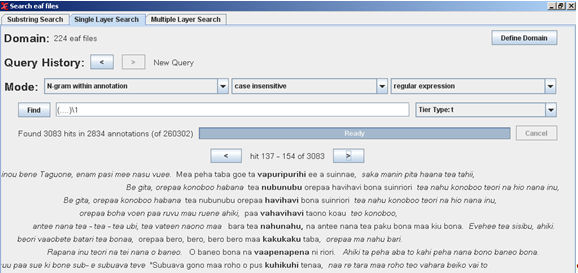
\includegraphics[width=.8\textwidth]{\imgpath/mosel-img3mod.png}
\end{center}
\caption{Search for reduplicated wordforms}
\label{fig:m10-1}
\end{figure}


Using more complex formulas you can restrict the search to forms with or without affixes in general or to forms with particular affixes as briefly illustrated in the appendix. But here I want to present one of my most complicated examples, namely the investigation of the noun-verb distinction in Teop, and discuss its problems.

Oceanic languages are well known for their presumably weak noun/verb distinction \citep{HengeveldEtAl2004,HengeveldEtAl2005}, but the investigation of lexical flexibility in Teop seems the first corpus-linguistic study of this phenomenon. The workflow of this investigation was as follows:

\begin{enumerate}
\item {Identify the elements constituting the constructional frames\footnote{Compare 
 the notions of collocational frame works, grammar patterns and colligates in \citet[936-937]{StefanowitschEtAl2009}. 
} 
of noun phrases (NPs) and verb complexes (VCs) - a constructional frame consists of functional morphs and empty, syntactically defined head and modifier positions for content words and stems).}
\item {Identify the functional elements that directly precede or follow the empty head position for the content word.}
\item {Construct Regular Expressions for the head position in NPs and VCs.}
\item {Select a few prototypical frequent action and object words e.g. `do, make', `say', `person', `thing', and search.}
\end{enumerate}

In Teop the constructional frames of NPs and VCs are quite complex. But for our purposes it was sufficient to construct the formulas that only include those functional elements that immediately precede either the head of NPs or the head of VCs, i.e. the articles, a plural marker, the numerals for `one' and 'two', and the diminutive particle for NPs and for the VC the pre-head tense, aspect and mood markers, the conjunction \textit{re} `so that, then', and the relative pronoun \textit{to}:
 
\ea \label{ex:m2} Regular expression for Teop NPs: \\
\texttt{
{\regexB}(a{\textbar}o{\textbar}bona{\textbar}bono{\textbar}peha{\textbar}peho{\textbar}bua{\textbar}buo{\textbar}amaa{\textbar}maa{\textbar}si){\regexB}
\newline
{\regexB}HEAD{\regexB}
}
\z



This formula means:
 
\ea \label{ex:m3} find any lexical form that is inserted in the HEAD position and preceded by 

\begin{itemize}
\item {the specific basic article \textit{a} or \textit{o} or }
\item {the object article \textit{bona }or \textit{bono}, or}
\item {the numeral \textit{peha, peho} `one' or \textit{bua, buo} `two',   or}
\item {the plural particle \textit{maa} or the complex form \textit{amaa} consisting of the article \textit{a} and the plural marker \textit{maa}, or}
\item {the diminutive particle \textit{si}. }
\end{itemize}
\z

\ea \label{ex:m4} Regular expression for Teop VCs

\texttt{
{\regexB}(are{\textbar}kahi{\textbar}na{\textbar}ore{\textbar}paa{\textbar}pasi{\textbar}re{\textbar}repaa{\textbar}tau{\textbar}to{\textbar}toro){\regexB} {\regexB}HEAD{\regexB}
}

\z

This formula means:


\ea \label{ex:m5} find any lexical form that is inserted in the HEAD position and preceded by

\begin{itemize}
\item {one of the six TAM markers \textit{kahi, na, paa, pasi, tau }or \textit{toro} or }
\item {the conjunction \textit{re} `then, so that' or }
\item {the relative pronoun \textit{to}, or }
\item {the conjunction \textit{re} with the 1inc.pl prefix \textit{a-} , i.e. \textit{are, }or  }
\item {the conjunction \textit{re} with the with 3sg/pl-prefix \textit{o-}, i.e. \textit{ore,} }
\item {or the conjunction \textit{re} `then, so that' with\textit{ }the suffixed TAM marker \textit{paa, }i.e. \textit{repaa}.%\footnote{Unfortunately 
%  the current version of ELAN 4.3.2 has problems to digest these long formulas so that I had to split them into two: For the heads of NPs I used
% \texttt{ ({\regexB}a{\regexB}{\textbar}{\regexB}o{\regexB}{\textbar}{\regexB}bona{\regexB}{\textbar}{\regexB}bono{\regexB}{\textbar}{\regexB}peha{\regexB}{\textbar}{\regexB}peho{\regexB}) {\regexB}HEAD{\regexB}}
% and 
% \texttt{
% ({\regexB}bua{\textbar}{\regexB}{\textbar}{\regexB}buo{\regexB}{\textbar}{\regexB}amaa{\regexB}{\textbar}{\regexB}maa{\regexB}{\textbackslash}{\textbar}{\regexB}si{\regexB}) {\regexB}HEAD{\regexB}
% }, 
% and for the heads of VCs  
% \texttt{({\regexB}are{\regexB}{\textbar}{\regexB}kahi{\regexB}{\textbar}{\regexB}na{\regexB}{\textbar}{\regexB}ore{\regexB}{\textbar}{\regexB}paa{\regexB}{\textbar}{\regexB}pasi{\regexB}) {\regexB}HEAD{\regexB}} 
% and 
% \texttt{({\regexB}re{\regexB}{\textbar}{\regexB}repaa{\regexB}{\textbar}{\regexB}tau{\regexB}{\textbar}{\regexB}to{\regexB}{\textbar}{\regexB}toro{\regexB}) {\regexB}HEAD{\regexB}.  }
% }
}
\end{itemize}
\z

These formulas do not cover the full range of possible contexts of NP and VC heads. The most notable exception is the very first position of the clause. In fast speech the speakers sometimes omit the article of NPs or the tense/aspect particle of a VC. Furthermore, imperatives are always unmarked for tense, aspect and mood and are not preceded by the conjunction \textit{re} or the relative pronoun \textit{to}. Consequently, the search with these formulas cannot reach the highest degree of coextensivity, but at least the readers are informed about the method and the limitations of the investigation, which contributes to the accountability of the grammatical description. 


A further problem is that some functional words are homonyms: the form \textit{na }represents a TAM marker and a portmanteau morph representing the 3pers.sg. possessive marker and the article of the following NP, and \textit{to} the relative pronoun preceding the VC and a rare non-specific article. This means that I either had to exclude these homonyms from my investigation or check all examples containing \textit{to} and \textit{na}. I opted for the latter, which was not too time consuming as the selected object words only rarely occurred with \textit{na} or \textit{to}. Had I chosen the first solution, the investigation would have been less coextensive, but would have still sufficed the accountability maxim as long as I documented my choice.  


The result of these searches was, as shown in the table below, that action words and object words are flexible with respect to the head positions in NPs and VCs, but that, as expected, action words are much more frequent in the VC head position and object words are much more frequent in the NP head position. Further research which employed the same kind of strategy revealed that action and object words are morpho-syntactically distinct in modifier positions so that verbs and nouns are formally distinct word classes in Teop, but at the same time show flexibility with respect to the NP and VC head positions, which contradicts Hengeveld, Rijkoff and Siewierska's (2004) theory of lexical flexibility.


Since I only investigated a few prototypical action and object words, my grammatical description is strictly speaking not adequate in coextensivity. This would only be the case if I had analysed and described all action and object words of the corpus, which would have been too time consuming and also unnecessary in my prototype approach. As I document the Regular Expressions of my searches, the readers can re-enact them and test the formulas with other head words.  

\begin{table}

\begin{tabular}{llllllll}

 &
 &
 VC head  &
 NP head  &
 &
 &
 VC head  &
 NP head \\
 \textit{asun}  &
 'hit, kill'  &
 70  &
 1  &
 \textit{aba}  &
 'person' &
 6 &
 243\\
 \textit{hua}  &
 'paddle'  &
 115  &
 4  &
 \textit{beiko}  &
 'child'  &
 1  &
 366 \\
 \textit{mosi}  &
 'cut'  &
 85 &
 9  &
 \textit{iana}  &
 'fish'  &
 {}-  &
 176 \\
 \textit{nao}  &
 'go'  &
 1002  &
 5  &
 \textit{moon}  &
 'woman'  &
 4  &
 665 \\
\itshape paku &
 'do, make' &
 996 &
 10 &
 \textit{naono}  &
 'tree'  &
 {}-  &
 136 \\
 \textit{pita}  &
 'walk'  &
 63 &
 3  &
 \textit{otei}  &
 'man'  &
 {}-  &
 478 \\
\itshape rosin &
 `flee' &
 211 &
 &
 \textit{taba}  &
 'thing'  &
 11  &
 461 \\
 \textit{sue}  &
 'say'  &
 752  &
 10  &
 \textit{vasu}  &
 'stone'  &
 {}- &
 48 \\
\end{tabular}
\caption{The distribution of typical verbs and nouns as heads of VCs and NPs}
\label{tab:m10-2}
\end{table}



With lexical items the problem of homonymy can easily be solved by simultaneous searches on the transcription and the translation tier. In order to distinguish, for instance, the adjective \textit{beera} `big, elder, important' from the noun \textit{beera} `chief' or the adjective \textit{beera} `chiefly', you only need to search for \textit{beera} on the transcription tier and its three translation equivalents on the translation tier.

\begin{figure}
\begin{center}
 
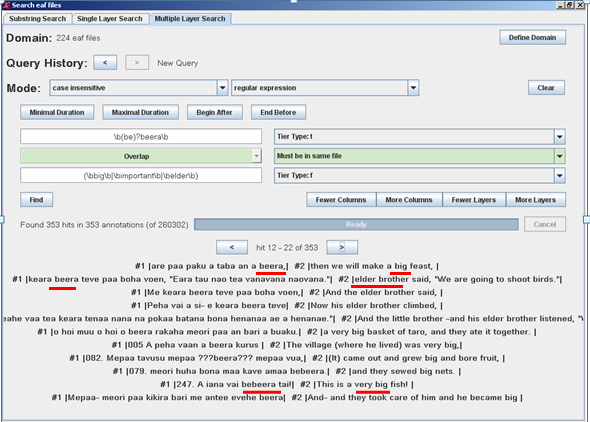
\includegraphics[width=.8\textwidth]{\imgpath/mosel-img4mod.png}
\caption{Search for \textit{beera }or \textit{bebeera }with the meaning `big', `important' or `elder'}
\end{center}

\label{fig:m10-2}
\end{figure}


If in the chapter on word classification I only gave the references for my examples, my description would be much less adequate in coextensivity, even if all of them were retrievable in the corpus because these few examples merely illustrate lexical flexibility, but do not demonstrate how my analysis and description actually relates to the corpus. Furthermore, the accountability of my description would be less scientific in view of the second maxim quoted above.


In the Teop Reference Grammar \citep{Moselinpreparation}   relatively simple and frequently used regular expressions as the one in Figure \ref{fig:m10-2} are described in an appendix, whereas the application of complex searches is documented in the endnotes of each chapter. In an electronic grammar each example could perhaps be linked to its particular Regular Expression formula which together with all other formulas would be stored in a single separate file. 

\section{Concluding remarks}%10.5 


Comparing my previous personal research methods with those of my current analysis of the Teop language, I am convinced that \citet{Whalen2004} was right when he assumed that ``the study of endangered languages will revolutionize linguistics.'' It is not only the way how we record speech by audio and video recordings, process the data in annotated digital corpora, make them globally accessible via the internet, and search them by the means of sophisticated query languages like Regular Expressions, but it is also the way how we - literally speaking - look at the data. Browsing through concordances as the ones depicted in Fig. 10.1 and Fig. 10.2 sharpens your eyes for regular patterns of language use and variation. It inspires you to create and test new formulas in your query language to either narrow down or extend your searches and thus explore the complex network of form-meaning correspondences in a hitherto unresearched language. With some practice you eventually ``think regular expressions'', as \citet[6]{Friedl2006} puts it, and understand how selected lexical units interact with certain constructions and, conversely, under which conditions selected constructions accommodate certain types of lexical units.


Unfortunately digital formats change so rapidly that digital archives cannot give long-term guarantees that they would continuously covert electronic grammars to new formats. Therefore I strongly recommend that the developers of electronic grammars provide for a function that facilitates the production of print outs and that these print-outs are stored in traditional libraries.

\newpage

\section{Appendix: Some useful regular expressions for ELAN users} 
This section only presents a very short introduction into what kind of searches can be done with regular expressions when analysing complex words or syntactic constructions. The best way to get started is just to try out what can be done with these formulas in your ELAN corpus or any other corpus that has implemented regular expressions. Note, however, that there are several dialects of this query language. For a comprehensive general introduction I recommend \citep{Friedl2006}. There is not yet any specialised investigation on the use of regular expressions in grammaticography.

\subsection{Symbols} \label{mosel:sec:71}
The following list only comprises a selection of those symbols that I found most useful. I tested them with Teop and German. 

\begin{table}[h]
\begin{tabular}{>{\tt}lp{4cm}p{4cm}}
\rm symbol &
place &
meaning\\
{\regexB} &
at the beginning and/or the end of a string &
word boundary\\
{\textbackslash}w+ &
at the end of a string &
variable end of word\\
. &
anywhere &
any letter\\
.* &
between spaces &
any string of letters between spaces/any word\\
.*{\textbackslash} &
between spaces &
any string of words \\
(x{\textbar}y) &
anywhere  &
either x or y\\
{}[\^{}x] &
place at the beginning &
not x\\
(....){\textbackslash}1 &
anywhere &
words with four reduplicated letters\\
? &
after a letter &
preceding letter is optional\\
(xyz)? &
anywhere &
the string xyz is optional\\
\end{tabular}
\caption{Symbols}
\end{table} 
 

\newpage
\subsection{Searching for particular complex word forms}
The symbols given in Section \ref{mosel:sec:71} can be combined for the search of morphologically complex words, especially for searches of words with particular suffixes or words containing reduplications. But the regular expressions do not recognise morpheme boundaries within a word.

\begin{table}[h]
\begin{tabular}{>{\tt}lp{3.5cm}p{4cm}}
\rm symbols &
hits &
examples\\
sa &
all words containing the string \textit{sa} &
\textit{sa, vasaku, sahata, tisa}\\
{\regexB}sa &
all words starting with \textit{sa} &
\textit{sa, sahata, sana, } NOT \textit{vasaku, tisa}\\
{\regexB}sa{\regexB} &
all words \textit{sa} &
\textit{sa}\\
{\regexB}sa..{\regexB} &
all words consisting of \textit{sa} and two letters that follow \textit{sa} &
\textit{saka, saku, sana,} \\
{\regexB}sa{\textbackslash}w+ &
all words beginning with \textit{sa,} but not \textit{sa} by itself &
\textit{sahata, sana}\\
{\regexB}.*ana{\regexB} &
all words ending in \textit{ana} &
\textit{sinana, tamuana, sana, bana, maana}\\
{\regexB}[\^{}(bana{\textbar}maana)].*ana{\regexB}

 &
all words ending in \textit{ana}, but not \textit{bana} or \textit{maana} &
\textit{sinana, tamuana, sana}\\
(....){\textbackslash}1 &
all words with four reduplicated letters &
\textit{pakupaku, vapakupaku,\newline
mahumahun, vamahumahun}\\
{\regexB}(....){\textbackslash}1 &
all words beginning with four reduplicated letters  &
\textit{pakupaku\newline
}NOT: \textit{vapakupaku}\\
{\regexB}(....){\textbackslash}1ana{\regexB} &
all words beginning with four reduplicated letters and ending in \textit{ana} &
\textit{vasuvasuana, hunuhunuana}\\
{\regexB}va(....){\textbackslash}1 &
all words with the prefix \textit{va-} and four reduplicated letters &
\textit{vapakupaku, vagunagunaha}\\
{\regexB}vahaa?{\regexB} &
all tokens of \textit{vahaa} and \textit{vaha} &
\textit{vahaa} and \textit{vaha}\\
\end{tabular}
\caption{Searching for particular complex word forms: Combinations of symbols on word level}
\end{table}
 
\newpage
\subsection{Searching for particular sequences of words}
\begin{table}[h]
\begin{tabular}{>{\tt}lp{3cm}p{5cm}}

\rm symbols &
hits &
examples\\

{\regexB}saka{\regexB} .* {\regexB}haa &
string of 3 words: 

(1) \textit{saka} 

(2) any word, and 

(3) the word \textit{haa} by itself or with suffixes &
\textit{saka antee haa;}

\textit{saka abana haari;}

\textit{saka kabuu haana}\\

saka .* {\regexB}haa{\textbackslash}w+ &
string of 3 words: 

(1) \textit{saka} 

(2) any word, and 

(3) a words beginning with \textit{haa}, \newline
but not \textit{haa} by itself &
\textit{saka abana haari};

\textit{saka kabuu haana}\\
 
{\regexB}(saka{\textbar}sa){\regexB} {\regexB}paku{\regexB}\newline
 &
all 2 word strings that consist of \textit{saka} or \textit{sa} and \textit{paku} &
\textit{saka paku, sa paku}\\


{\regexB}(saka{\textbar}sa){\regexB} .* {\regexB}vaha{\regexB} &
all 3 word strings with 

(1) \textit{saka} or \textit{sa}, 

(2) any word

(3) \textit{vaha}  &
\textit{saka tii vaha}

\textit{sa tapaku vaha}\\


{\regexB}(saka{\textbar}sa){\regexB} (....){\textbackslash}1 {\regexB}haa &
all 3 word strings with 

(1) \textit{saka} or \textit{sa}, 

(2) a word with four reduplicated letters

(3) the word \textit{haa} or a word beginning with \textit{haa} &
\textit{sa natanata haa},

\textit{ saka natanata haana}\\
\end{tabular}
\caption{Searching for particular sequences of words: Combinations of  the symbols  {\regexB}, \texttt{.*. {\textbackslash}w+ and (x{\textbar}y)}}
\label{mosel:tab:3}
\end{table} 

Comments on Table \ref{mosel:tab:3}:

\textit{saka/sa} ... \textit{haa} is a discontinuous negation. The last component \textit{haa} can have a suffix that indicates imperfective aspect and person, e.g. \textit{haana, haari, haara.} The formulas above provide data for the following questions:

\begin{enumerate}
\item Which words are used inbetween \textit{saka} and \textit{haa/haana/haari/haara}?
\item Which words are used inbetween \textit{saka} and \textit{haana/haari/haara} ?
\item Are there examples for \textit{saka/sa} followed by \textit{paku} `do'?
\item Which words are used between \textit{saka/sa} and \textit{vaha} `back, also, again, anymore'?
\item Does \textit{saka/sa ... haa} combine with reduplicated words?
\end{enumerate}

\subsection{Multilayer search with regular expressions}

Multilayer search is useful if you want to find examples of a homonymous lexical item or functional word as, for instance, the Teop non-specific article \textit{ta} `any, some' which is homonymous with the noun \textit{ta} `part' and the complementizer \textit{ta.}When I came across a sentence in which this non-specific article was followed by the demonstrative pronoun \textit{vai} `this' and a relative clause introduced by \textit{to}, I searched for all examples of this extraordinary construction 

\ea
\gll ta ....  X vai to \\
     \textsc{art} .... X \textsc{dem} \textsc{rel} \\
      `any/some ... X that'
\z

in the corpus using the formula
\texttt{
 {\regexB}ta{\regexB} .*{\textbackslash} {\regexB}vai{\regexB} {\regexB}to{\regexB}
}
 on the transcription tier and \texttt{(any{\textbar}some)} on the translation tier:


\begin{figure}[h]
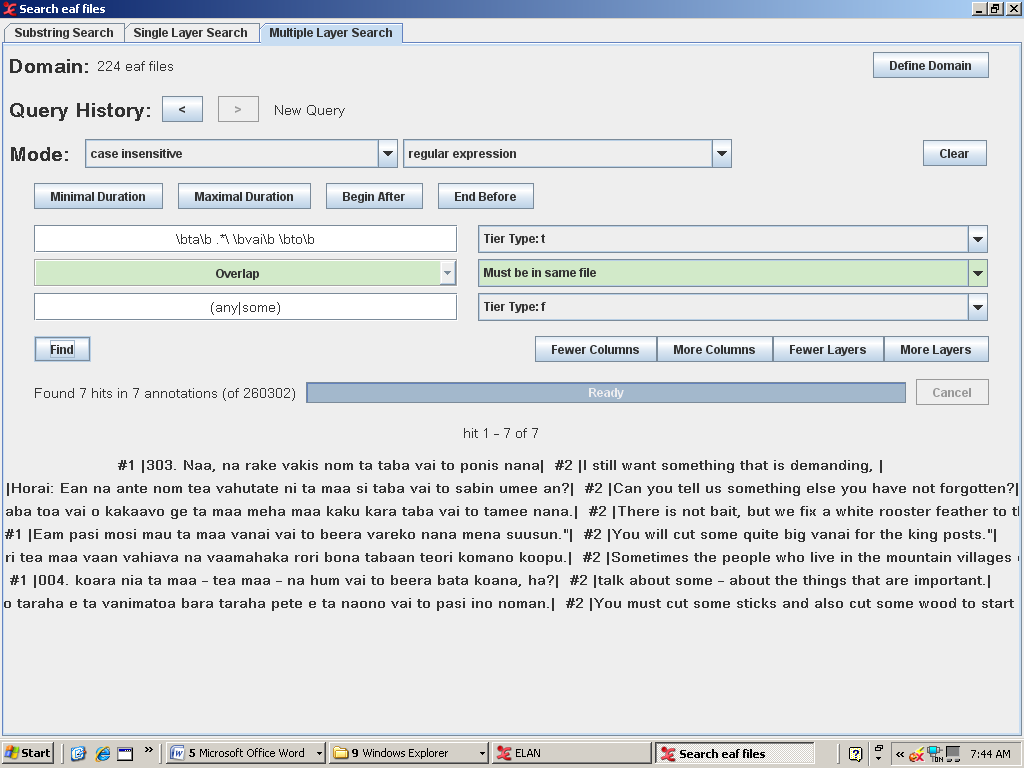
\includegraphics[width=\textwidth]{\imgpath/appendix-img3.png}
 
\caption{Multilayer search for \textit{ta} with the translation `any' or `some'}
\end{figure}

This formula means: search within an annotation for all occurences of \textit{ta} meaning `any' or `some' that is first followed by one or more unspecified words and then by the demonstrative \textit{vai} and the relative pronoun \textit{to}. 

Multilayer search is also practical, if you do not know the language well and want to search for a word and all its translations. Then you search on the free translation tier with the wild card .* For example, the search for \textit{mararae} gives you the translations `happy', `joyful' and `joy'.

\begin{figure}[h]
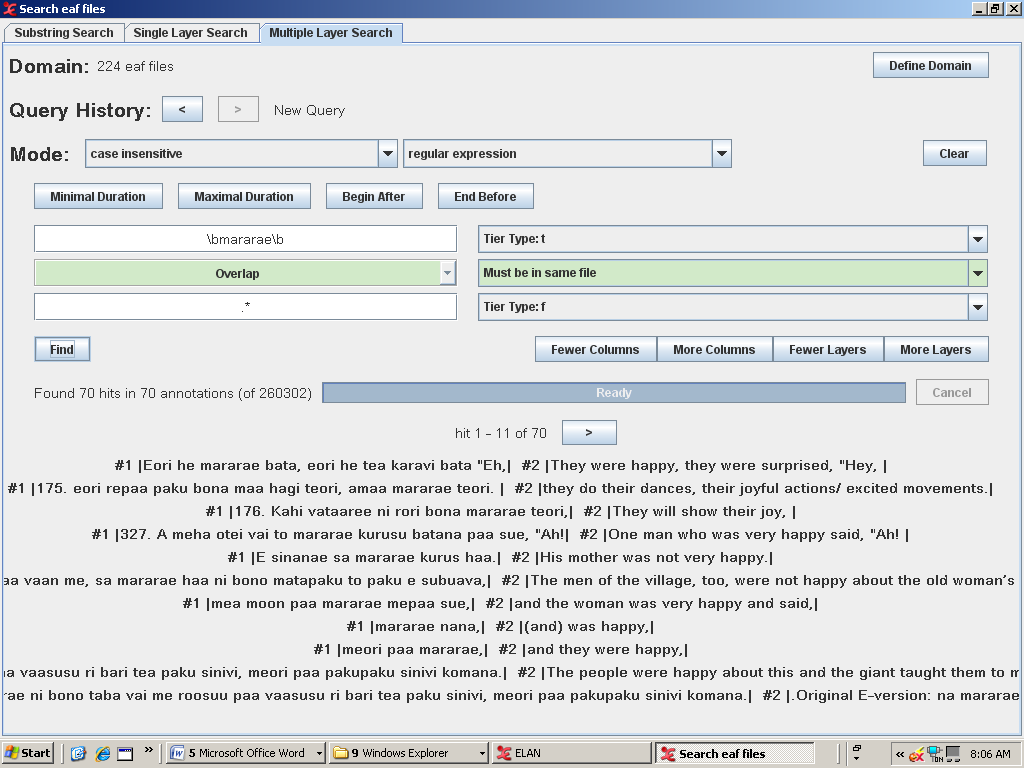
\includegraphics[width=\textwidth]{\imgpath/appendix-img4.png}
\caption{Multilayer search for \textit{mararae} with any translation}
\end{figure}
